\documentclass{article}
\usepackage{graphicx} % Required for inserting images

\title{Quantum Tomography Stats Model}
\date{May 2023}
\usepackage{braket}
\usepackage{amsmath}
\usepackage{mathtools}
\usepackage{amssymb}
\usepackage{multicol}
\usepackage{hyperref}

\begin{document}

\maketitle

\newcommand{\Like}{\mathcal{L}}
\newcommand{\EX}{\mathbb{E}}
\newcommand{\Tr}[1]{\operatorname{Tr}\left(#1\right)}

\section{Introduction}
Given the measurement data we wish to determine the best possible estimate for the quantum state. We can use \href{https://en.wikipedia.org/wiki/Bayes%27_theorem}{Bayes' theorem} to define the probability of the state given the data:

$$\text{Pr}(\rho|\text{Data}) = \frac{\text{Pr}(\text{Data}|\rho)\text{Pr}(\rho)}{\text{Pr}(\text{Data})} \;.$$

We define these functions as the following
\begin{itemize}
\item Posterior:  $\text{Pr}(\rho|\text{Data})$
\item Likelyhood: $\Like(\rho) = \text{Pr}(\text{Data}|\rho)$
\item Prior:      $\text{Pr}(\rho)$
\item Evidence:   $\text{Pr}(\text{Data})$
\end{itemize}

\section{Distribution of Counts}
The counts of the measurements can be modeled by a \href{https://en.wikipedia.org/wiki/Poisson_distribution}{Poisson Distrobution}. With high enough counts we can approximate this with a \href{https://en.wikipedia.org/wiki/Normal_distribution}{Normal Distrobution} using the \href{https://en.wikipedia.org/wiki/Central_limit_theorem}{Central Limit Theorm}. A important fact of the poisson distrobution is the variance is equal to the mean.

\section{1det/qubit}
For each measurement we have 1 count number. From the \href{http://research.physics.illinois.edu/QI/Photonics/tomography-files/amo_tomo_chapter.pdf}{Photonic State Tomography} paper, the distribution of the counts follows:

$$n_i \sim \text{Poiss}(\mu_{i}) \xrightarrow{\text{CLT}}
       n_i \sim \text{Norm}(\mu_{i},\sigma_i) \;,$$
$$\mu_{i} = I_0 I_i \Tr{ M'_i \rho } + a_i \;.$$

\subsection{Variables: }
\begin{itemize}
\item $n_i$: Number of counts on measurement i
\item $\mu_i$: Expected number of counts on measurement i given $\rho$
\item $i \in[1,m] \; \big| \; m = \text{Number of Measurements}$
\item $\sigma_i^2$: Variance for the number of counts on measurement i given $\rho$
\begin{itemize}
    \item $\sigma_i^2 = \mu_i$ from assuming a poisson distribution
\end{itemize}
\item $I_0$: Is the overall intensity
\item $I_i$: Is the relative intensity of measurement i given as an input. Default is 1
\item $M'_i$: Is measurement i with cross talk correction
\item $a_i$ : Is the predicted accidental counts for measurement i.
\end{itemize}

\subsection{Log-Likelyhood}
$$\Like(\rho) = \text{Pr}(\text{Data}|\rho) \;,$$
$$\Like(\rho) = \prod_{i=1}^m \text{Pr}(n_i|\mu_i)$$
$$\Like(\rho) = \prod_{i=1}^m \frac{1}{\sqrt{\sigma_i2\pi}}
                \exp\left( -\frac{(n_i-\mu_i)^2}{2\sigma_i^2} \right)$$

The $\frac{1}{\sqrt{\sigma_i2\pi}}$ is a normalization factor. Since we are maximizing this
function we can ignore this term

$$\Like(\rho) \propto \prod_{i=1}^m \exp\left( -\frac{(n_i-\mu_i)^2}{2\sigma_i^2} \right)$$

We can plug in $\sigma_i^2 = \mu_i$ and take the log of this function to get our log-Likelyhood function.

$$\text{log}(\Like(\rho)) = \sum_{i=1}^m -\frac{(n_i-\mu_i)^2}{2\mu_i^2}$$

\section{2det/qubit}
For each measurement a complete number of counts on all the possible outcomes. We define the following variables:

From the \href{http://research.physics.illinois.edu/QI/Photonics/tomography-files/amo_tomo_chapter.pdf}{Photonic State Tomography} paper:

$$n_{ij} \sim \text{Poiss}(\mu_{ij}) \xrightarrow{\text{CLT}} n_{ij} \sim \text{Norm}(\mu_{ij},\sigma_{ij})\;,$$
$$\mu_{ij} = I_0 I_i E_j \Tr{ M'_{ij} \rho } + a_{ij}\;.$$

\subsection{Variables}

\begin{itemize}
\item $n_{ij}$: Number of counts on measurement i for detector j
\item $\mu_{ij}$: Expected number of counts on measurement i, detector j  given $\rho$
\item $i \in[1,m] \; \big| \; m = \text{Number of Measurements}$
\item $j \in[1,k] \; \big| \; k = \text{Number of Detector Pairs}$
\item $\sigma_{ij}^2$: Variance for the number of counts on measurement i, detector j given $\rho$
\begin{itemize}
    \item  $\sigma_{ij}^2 = \mu_{ij}$ from assuming a poisson distribution
\end{itemize}
\item $I_0$: Is the overall intensity
\item $I_i$: Is the relative intensity of measurement i given as an input. Default is 1
\item $E_j$ Is the relative efficiency on the jth basis
\item $M'_{ij}$: Is the jth basis of measurement i with cross talk correction
\end{itemize}

\subsection{Log-Likelyhood}

$$\Like(\rho) = \text{Pr}(\text{Data}|\rho)$$
$$\Like(\rho) = \prod_{i=1}^m \prod_{j=1}^k  \text{Pr}(n_{ij}|\mu_{ij})$$
$$\Like(\rho) = \prod_{i=1}^m \prod_{j=1}^k  \frac{1}{\sqrt{\sigma_{ij}2\pi}}
                \exp\left( -\frac{(n_{ij}-\mu_{ij})^2}{2\sigma_{ij}^2} \right)$$

The $\frac{1}{\sqrt{\sigma_{ij}2\pi}}$ is a normalization factor. Since we are maximizing this
function we can ignore this term

$$\Like(\rho) \propto \prod_{i=1}^m \prod_{j=1}^k  \exp\left( -\frac{(n_{ij}-\mu_{ij})^2}{2\sigma_{ij}^2} \right)$$

We can plug in $\sigma_{ij}^2 = \mu_{ij}$ and take the log of this function to get our log-Likelyhood function.

$$\text{log}(\Like(\rho)) = \sum_{i=1}^m  \sum_{j=1}^k -\frac{(n_{ij}-\mu_{ij})^2}{2\mu_{ij}^2}$$


\section{Error Correction}

\subsection{Accidental Correction}

Accidental Correction is used for 2 detectors per qubit.

$$a_{ij} = \frac{W_j}{T_i * 10^9}\prod_{k=1}^{2}S_{ijk}$$

\begin{itemize}
\item $T_i$ Is the time in nanoseconds of measurement i given as an input. Default is 1
\item $S_{ijk}$ Is the kth single count on measurement i given as an input. Default is 0
\item $W_j$ Is the coincidence window duration for the jth basis as an input. Default is 0
\end{itemize}

\subsection{Crosstalk}

$$M'_{i,j} = \sum_{j'=1}^{k} C_{j,j'} M_{i,j}$$

\begin{itemize}
\item $M'_{ij}$: Is the jth basis of measurement i with cross talk correction
\item $M_{ij}$: Is the jth basis of measurement i.The state the target quantum state is projected on. These are pure states here represented as density matrices
\item $C_{ij}$: The index at the jth row and j'th column of the crosstalk matrix
\item $i \in[1,m] \; \big| \; m = \text{Number of Measurements}$
\item $j,j' \in[1,k] \; \big| \; k = \text{Number of Detector Pairs, which is equal to the number of qubits squared.}$
\end{itemize}

\section{Lab setup example: 2 qubits with 2 det/qubit vs 1 det/qubit}
We need to specify 2 states per measurement. The first is the state that the first qubit is projected onto when it ends up at detector 1. The second is the state that the second qubit is projected onto when it ends up at detector 2.

\begin{multicols}{2}
\textbf{2det/qubit}
\begin{enumerate}
  \item Det-pair 1 : 1-2
  \item Det-pair 2 : 1-4
  \item Det-pair 3 : 3-2
  \item Det-pair 4 : 3-4
\end{enumerate}

\columnbreak

\textbf{1det/qubit}
\begin{enumerate}
  \item Det-pair 1 : 1-2
\end{enumerate}

\end{multicols}


\begin{center}
    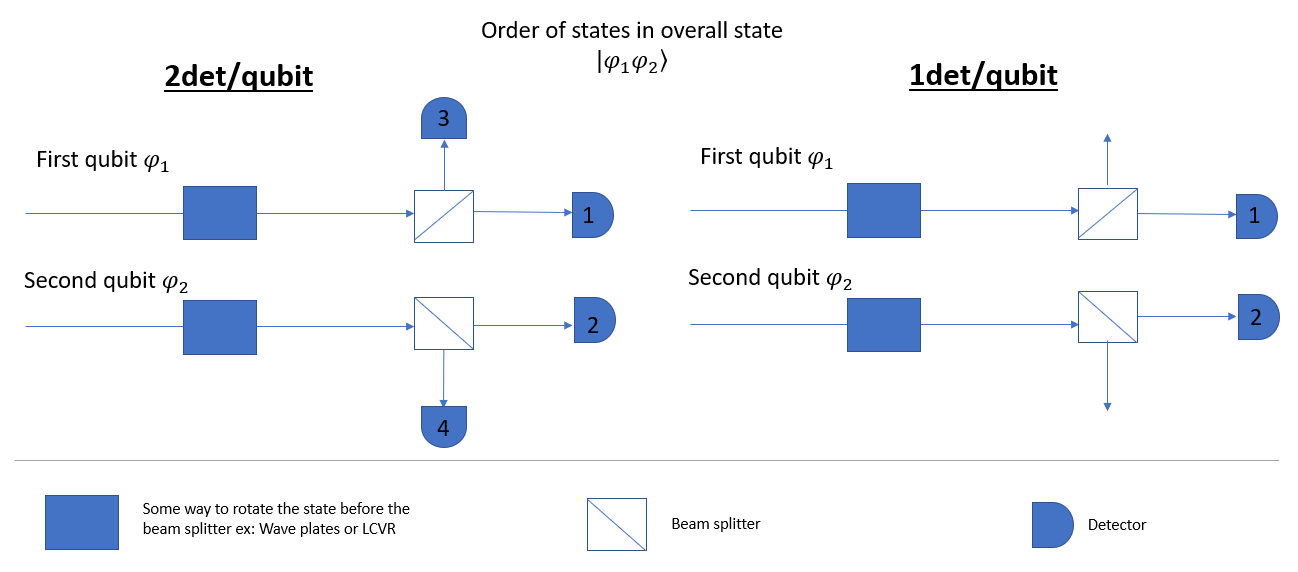
\includegraphics[scale=.6]{DetectorPairs}
\end{center}



\section{Estimators}

\subsection{Maximum Likelyhood Estimator(MLE)}
The MLE estimator is found by maximizing the log of the likelyhood function:

$$\rho_\text{MLE} =
\operatorname*{argmin}_{\rho} -\text{log}(\Like(\rho)) \; .$$

\subsection{Hedged Maximum Likelyhood Estimator(HMLE)}
Hedged maximum likelihood is a simple modification of the maximum likelihood approach. Instead of maximizing the likelihood, the estimate is the one that maximizes the product of the likelihood with the following hedge function:
$$h(\rho)=\operatorname{det}(\rho)^{\beta} \mid \beta \in\left[0, \frac{1}{2}\right] \;,$$
$$\rho_{\mathrm{HMLE}}=\underset{\rho}{\operatorname{argmin}}-\log (\mathcal{L}(\rho) h(\rho)) \;.$$

The value of Beta can be defined in the conf settings; default is 1/2. Robin Blume-Kohout covers the hedged likelihood function in more detail in the paper titled [Hedged Maximum Likelihood Estimation](https://arxiv.org/pdf/1001.2029.pdf).

\subsection{Bayesian Estimator(BME)}
The Bayes estimator is the expected value of the posterior

$$\hat{\rho}_\text{BME} = \EX_\text{posterior}[\rho | \text{Data}]$$
$$\hat{\rho}_\text{BME} = \int\rho\text{Pr}(\rho|Data) d\rho$$
$$\hat{\rho}_\text{BME} =  \int\rho \frac{\text{Pr}(\text{Data}|\rho)\text{Pr}(\rho)}{\text{Pr}(\text{Data})} d\rho$$

We only care about an estimator that is proportional to the density matrix since we can normalize the matrix at the end.

$$\hat{\rho}_\text{BME} \propto \int\rho\text{Pr}(\text{Data}|\rho)\text{Pr}(\rho) d\rho$$
$$\hat{\rho}_\text{BME} \propto \EX_\text{prior}[\rho\text{Pr}(\text{Data}|\rho)]$$

Monte Carlo Approximation of the Bayesian Estimator
$$\hat\rho_\text{BME}
=       \EX_\text{posterior}[\rho | \text{Data}]
\propto \EX_\text{prior}[\rho\text{Pr}(\text{Data}|\rho)]$$

$\rho_i \sim \text{Pr}(\rho)$ is a random sample from the prior
$$\hat\rho_\text{BME} \propto \sum_i \rho_i\text{Pr}(\text{Data}|\rho)$$

$\rho_i \sim \text{Pr}(\rho | \text{Data})$ is a random sample from posterior
$$\hat\rho_\text{BME} \propto \sum_i \rho_i$$

\section{Linear Inversion}
The Linear Inversion method is a simpler approach to State Tomography. It is used to get a starting state for MLE and is typically not recommended on its own as it can give non-valid density matrices.
\subsection{1 Qubit}
We can represent any density matrix in terms of the stokes parameters and the pauli matrices.
$$
\sigma_0 = \begin{bmatrix}1 & 0\\0 & 1 \end{bmatrix} \;
\sigma_1 = \begin{bmatrix}0 & 1\\1 & 0 \end{bmatrix} \;
\sigma_1 = \begin{bmatrix}0 & i\\i & 0 \end{bmatrix} \;
\sigma_3 = \begin{bmatrix}1 & 0\\0 &-1 \end{bmatrix} \;$$
$$\rho = \frac{1}{2}\sum_{i=0}^3 S_i \sigma_i \;\bigg|\; S_i = \Tr{\rho\sigma_i} $$
$$\rho = \frac{1}{2}\vec{S}_\rho \cdot \vec{\sigma} 
\;\bigg|\; 
\vec{\sigma} = \begin{bmatrix}\sigma_0 \\ \sigma_1 \\ \sigma_2 \\ \sigma_3\end{bmatrix},
\vec{S}_\rho = \begin{bmatrix}\Tr{\rho\sigma_0} \\ \Tr{\rho\sigma_1} \\ \Tr{\rho\sigma_2} \\ \Tr{\rho\sigma_3}\end{bmatrix}$$

For a general set of projectors $\{M_i\}$, the probability that $\rho$ will collapse to $M_i$ is $P_i = \Tr{M_i\rho}$.

$$\vec{P} 
= \begin{bmatrix} \Tr{M_0\rho} \\ \Tr{M_1\rho} \\ \vdots \\ \Tr{M_{m-1}\rho} \end{bmatrix}
= \begin{bmatrix} 
\Tr{M_0\left(\frac{1}{2}\sum_{j=0}^3 S_j \sigma_j\right)} \\
\Tr{M_1\left(\frac{1}{2}\sum_{j=0}^3 S_j \sigma_j\right)} \\ 
\vdots \\ 
\Tr{M_{m-1}\left(\frac{1}{2}\sum_{j=0}^3 S_j \sigma_j\right)} 
\end{bmatrix}
= \begin{bmatrix} 
\frac{1}{2}\sum_{j=0}^3\Tr{M_0\sigma_j}S_j \\
\frac{1}{2}\sum_{j=0}^3\Tr{M_1\sigma_j}S_j \\ 
\vdots \\ 
\frac{1}{2}\sum_{j=0}^3\Tr{M_{m-1}\sigma_j} S_j
\end{bmatrix}$$

Define the matrix $\textbf{B} \;\big|\; B_{ij} = \Tr{M_i\sigma_j}$

$$\vec{P} = \textbf{B} \vec{S_{\rho}}$$

Finally we use the psuedo-inverse to get $\vec{S_{\rho}}$:

$$
\begin{aligned}
\vec{P} &= \textbf{B} \vec{S_{\rho}} \\
\textbf{B}^T\vec{P} &= \textbf{B}^T\textbf{B} \vec{S_{\rho}} \\
(\textbf{B}^T\textbf{B})^{-1}\textbf{B}^T\vec{P} &= \vec{S_{\rho}} \\
\end{aligned}
$$

Our probability vector can be approximated by our counts
\subsection{N Qubits}
This can easily be scaled to larger dimensions. We simply scale the pauli basis by doing:

$$\vec{\sigma} = 
\bigotimes_{n=1}^N \begin{bmatrix}\sigma_0 \\ \sigma_1 \\ \sigma_2 \\ \sigma_3\end{bmatrix}$$
$$\rho = \frac{1}{2^N}\sum_{i=0}^{4^N-1} S_i \sigma_i \;\bigg|\; S_i = \Tr{\rho\sigma_i} $$
For example, for 2 qubits our pauli basis would be
$$\vec{\sigma} = \begin{bmatrix}
\sigma_0\otimes\sigma_0 \\ \sigma_0\otimes\sigma_1 \\ \sigma_0\otimes\sigma_2 \\ \sigma_0\otimes\sigma_3 \\
\sigma_1\otimes\sigma_0 \\ \sigma_1\otimes\sigma_1 \\ \sigma_1\otimes\sigma_2 \\ \sigma_1\otimes\sigma_3 \\
\sigma_2\otimes\sigma_0 \\ \sigma_2\otimes\sigma_1 \\ \sigma_2\otimes\sigma_2 \\ \sigma_2\otimes\sigma_3 \\
\sigma_3\otimes\sigma_0 \\ \sigma_3\otimes\sigma_1 \\ \sigma_3\otimes\sigma_2 \\ \sigma_3\otimes\sigma_3 \\
\end{bmatrix}^$$

\section{Parameterization}
During the optimization we parameterize the density matrix as follows in order to ensure we are only considering valid density matrices:

$$\rho=T T^{\dagger} \;,$$
$$T=\begin{bmatrix}
t_{1} & 0 & \ldots & 0 \\
t_{2^{n}+1}+i t_{2^{n}+2} & t_{2} & \ldots & 0 \\
\ldots & \ldots & \ldots & 0 \\
t_{4^{n}-1}+i t_{4^{n}} & t_{4^{n}-3}+i t_{4^{n}-2} & t_{4^{n}-5}+i t_{4^{n}-4} & t_{2 n}
\end{bmatrix}\;.$$

\end{document}
